\subsubsection{PageRank}

The experiment result (Figure. \ref{fig:pagerank}) shows that the Pagerank value distribution in most of graphs follow power law.

\begin{figure}
\subfloat[as-skitter.75000\label{fig:as-skitter}]
  {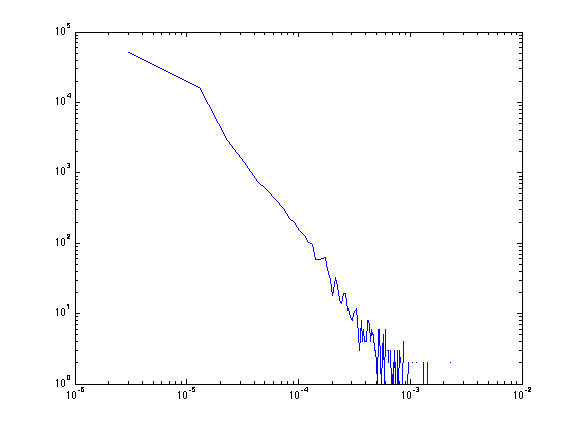
\includegraphics[width=.25\linewidth]{FIG/pagerank/as-skitter_75000.png}}\hfill
\subfloat[ca-AstroPh\label{fig:ca-AstroPh}]
  {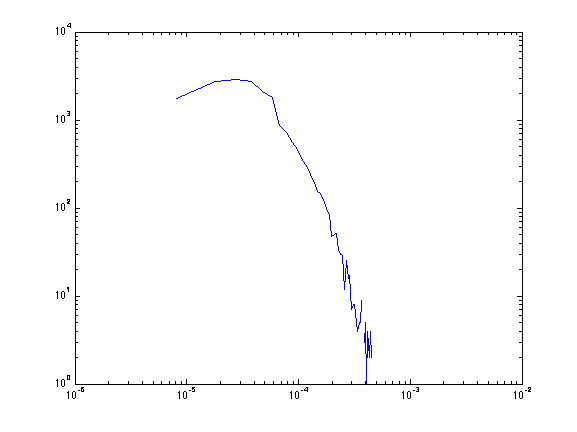
\includegraphics[width=.25\linewidth]{FIG/pagerank/ca-AstroPh.png}}\hfill
\subfloat[cit-HepPh\label{fig:cit-HepPh}]
  {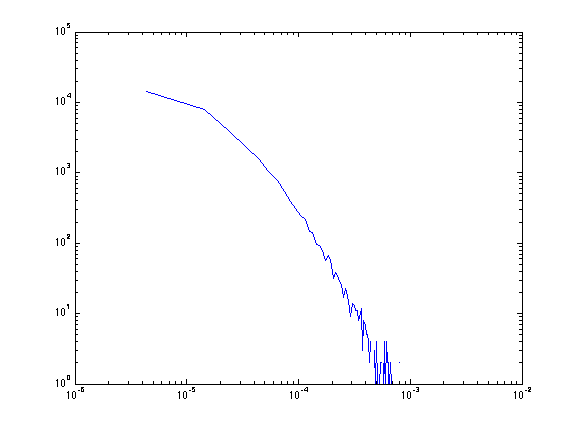
\includegraphics[width=.25\linewidth]{FIG/pagerank/cit-HepPh.png}} \hfill
\subfloat[cit-HepTh\label{fig:cit-HepTh}]
  {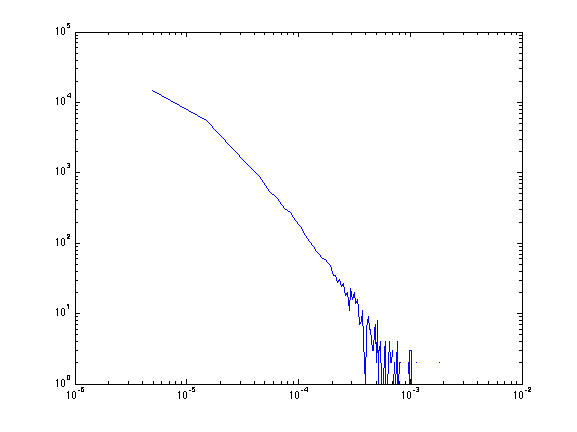
\includegraphics[width=.25\linewidth]{FIG/pagerank/cit-HepTh.png}}\hfill
\subfloat[com-amazon.ungraph-75000\label{fig:com-amazon.ungraph-75000}]
  {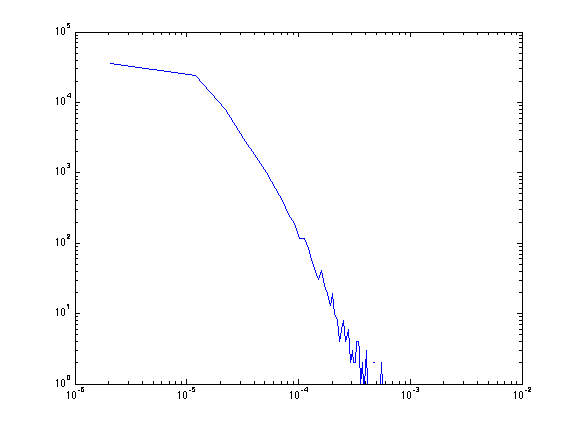
\includegraphics[width=.25\linewidth]{FIG/pagerank/com-amazon.ungraph-75000.png}}\hfill
\subfloat[com-dblp.ungraph-75000\label{fig:com-dblp.ungraph-75000}]
  {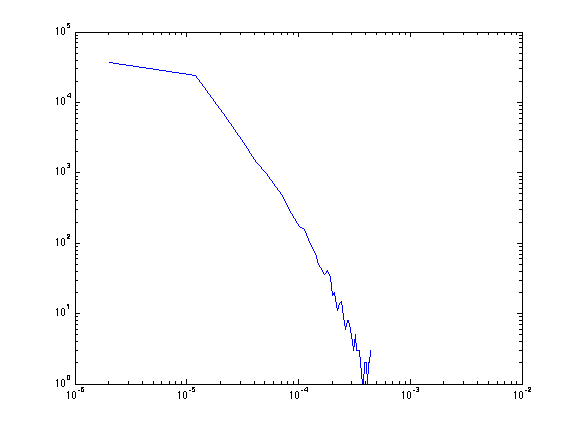
\includegraphics[width=.25\linewidth]{FIG/pagerank/com-dblp.ungraph-75000.png}} \hfill
 \subfloat[email-Enron.ungraph\label{fig:email-Enron.ungraph}]
  {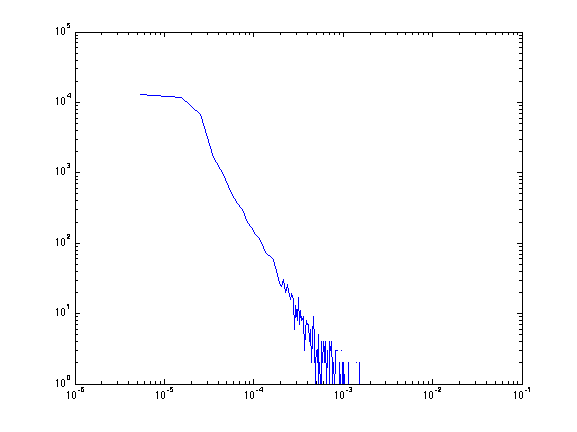
\includegraphics[width=.25\linewidth]{FIG/pagerank/email-Enron.ungraph.png}}\hfill
\subfloat[email-EuAll\label{fig:email-EuAll}]
  {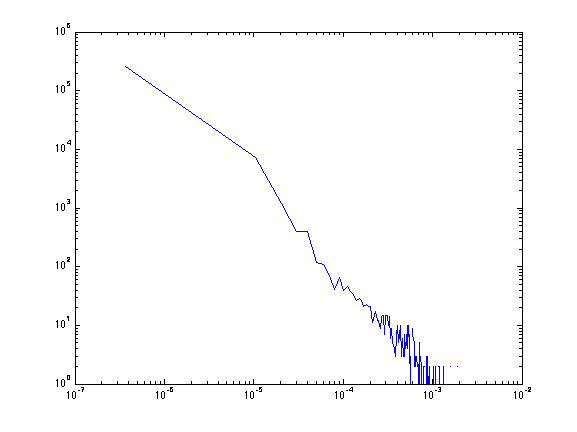
\includegraphics[width=.25\linewidth]{FIG/pagerank/email-EuAll.png}}\hfill
\subfloat[p2p-Gnutella31\label{fig:p2p-Gnutella31}]
  {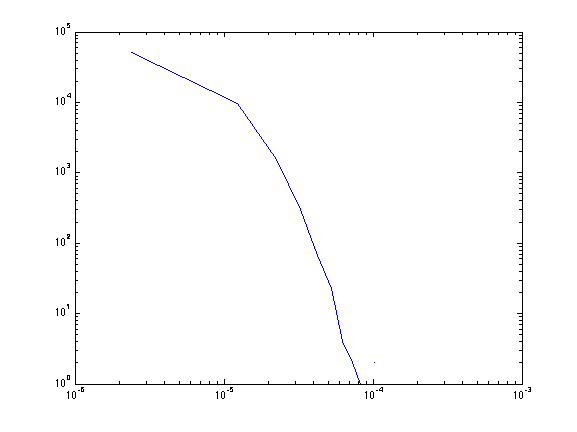
\includegraphics[width=.25\linewidth]{FIG/pagerank/p2p-Gnutella31.png}} \hfill
 \subfloat[soc-Slashdot0811-75000\label{fig:soc-Slashdot0811-75000}]
  {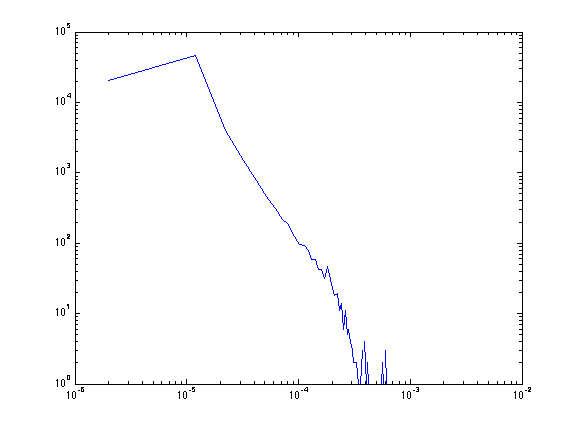
\includegraphics[width=.25\linewidth]{FIG/pagerank/soc-Slashdot0811-75000.png}} 
 \subfloat[as-Caida\label{fig:as-Caida}]
  {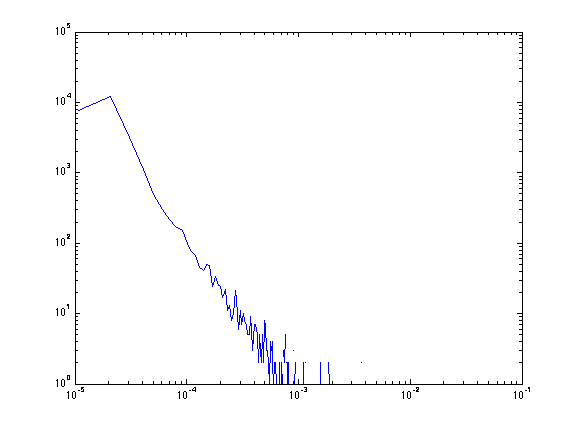
\includegraphics[width=.25\linewidth]{FIG/pagerank/as-Caida.undir.txt.png}} \hfill  
 \subfloat[bio-protein\label{fig:bio-protein}]
  {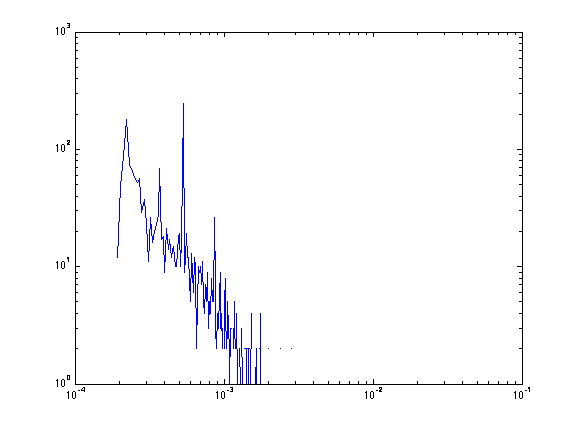
\includegraphics[width=.25\linewidth]{FIG/pagerank/bio-protein-undir.txt.png}} \hfill  
 \subfloat[cit-Cora\label{fig:cit-Cora}]
  {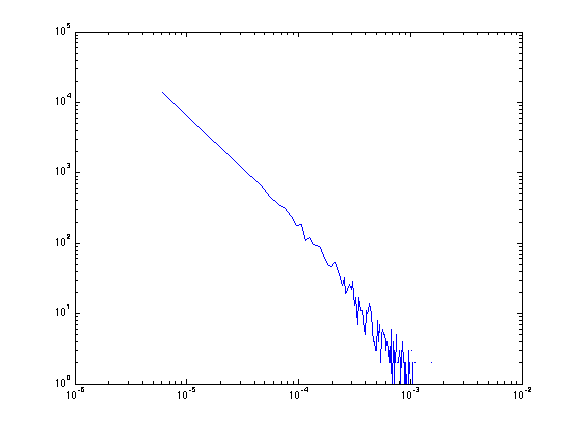
\includegraphics[width=.25\linewidth]{FIG/pagerank/cit-Cora.txt.png}} \hfill 
 \subfloat[soc-digg\label{fig:soc-digg}]
  {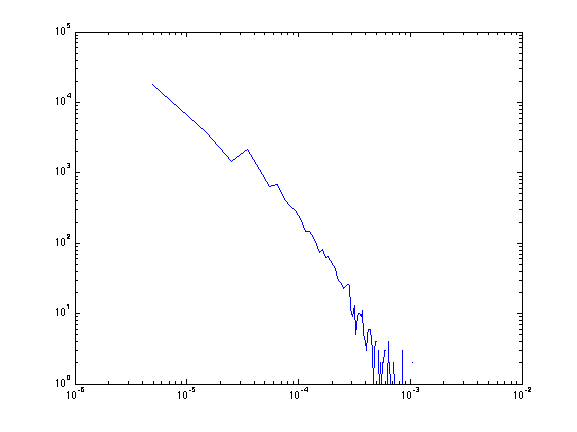
\includegraphics[width=.25\linewidth]{FIG/pagerank/soc-digg.txt.png}} \hfill  
 \subfloat[soc-flickr-75000\label{fig:soc-flickr-75000}]
  {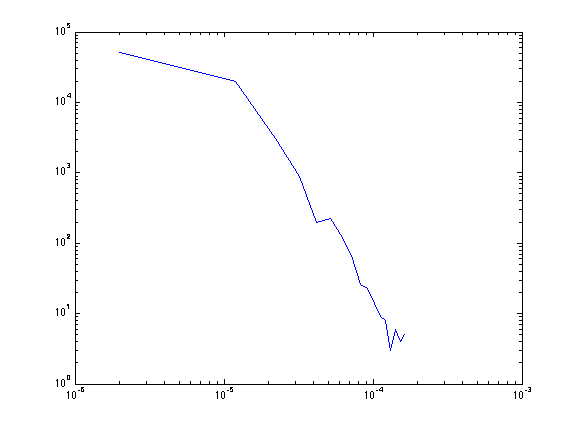
\includegraphics[width=.25\linewidth]{FIG/pagerank/soc-flickr-75000.txt.png}} \hfill  
 \subfloat[soc-hamsterster\label{fig:soc-hamsterster}]
  {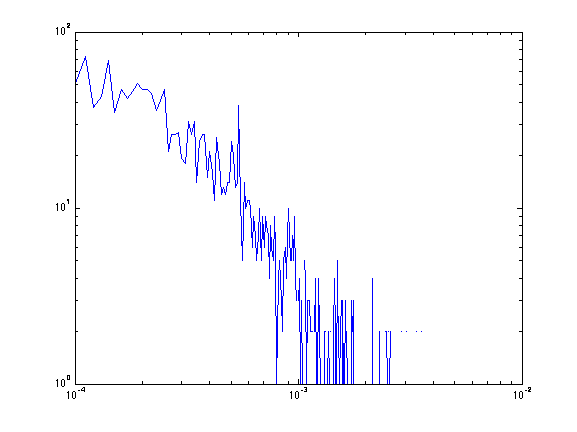
\includegraphics[width=.25\linewidth]{FIG/pagerank/soc-hamsterster.undir.txt.png}} \hfill  
 \subfloat[soc-pokec-75000\label{fig:soc-pokec-75000}]
  {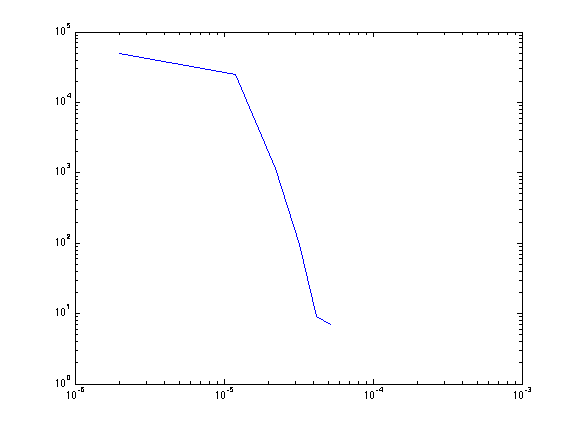
\includegraphics[width=.25\linewidth]{FIG/pagerank/soc-pokec-75000.txt.png}} \hfill  
 \subfloat[soc-Youtube-75000\label{fig:soc-Youtube-75000}]
  {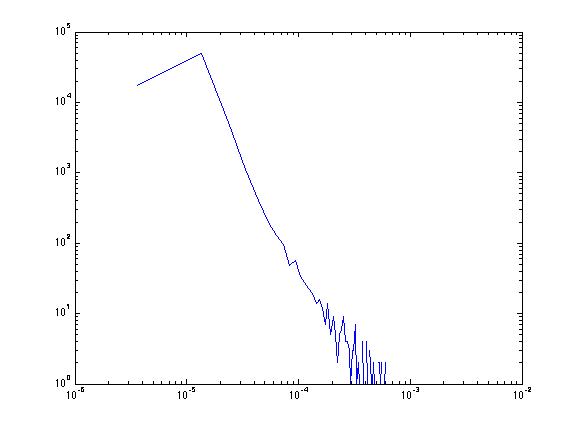
\includegraphics[width=.25\linewidth]{FIG/pagerank/soc-Youtube-75000.undir.txt.png}} \hfill  
 \subfloat[soft-jdkdependency\label{fig:soft-jdkdependency}]
  {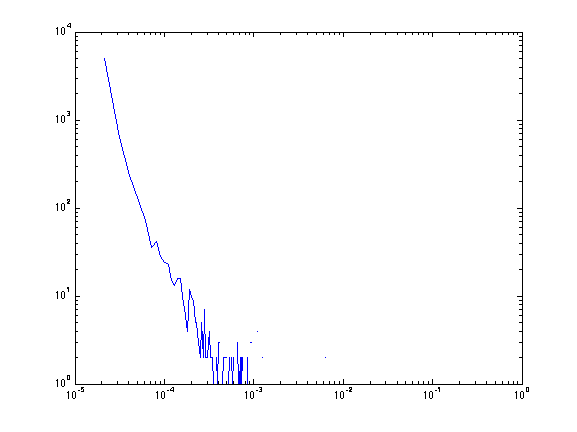
\includegraphics[width=.25\linewidth]{FIG/pagerank/soft-jdkdependency.txt.png}} \hfill  
 \subfloat[text-spanishbook\label{fig:text-spanishbook}]
  {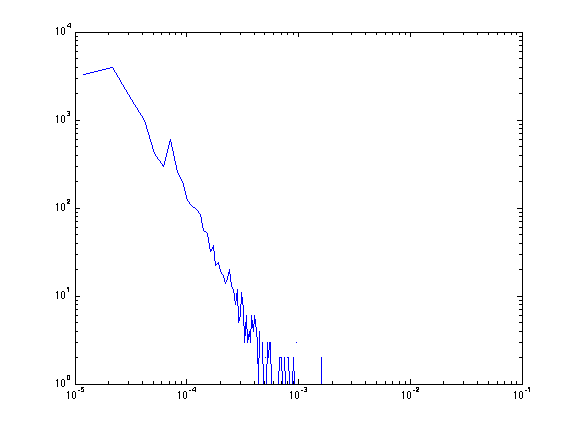
\includegraphics[width=.25\linewidth]{FIG/pagerank/text-spanishbook.txt.png}} \hfill  
\caption{Pagerank value Distributions of 20 graphs}
\label{fig:pagerank}
\end{figure}